\documentclass[a4paper,11pt]{article}
\usepackage{geometry}
\geometry{margin=1in}
\usepackage{graphicx}
\usepackage{amsmath}
\usepackage{hyperref}
\usepackage{float}
\usepackage{caption}
\usepackage{booktabs}
\usepackage{cleveref}
\hypersetup{
    colorlinks=true,
    linkcolor=blue,
    filecolor=magenta,
    urlcolor=cyan,
    pdftitle={Stress Concentrations in Solid Mechanics},
    pdfauthor={Your Full Name},
    bookmarksopen=true,
    bookmarksnumbered=true
}
\usepackage{pgfplots}
\pgfplotsset{compat=1.17}
\begin{figure}[h!]
    \centering
    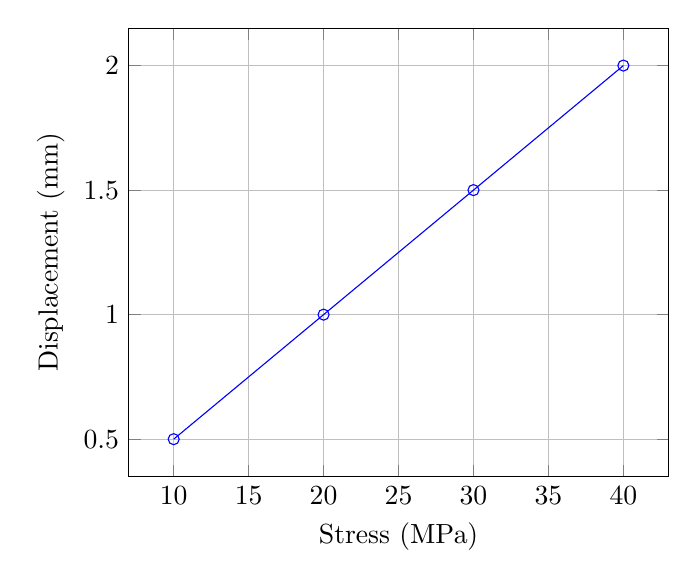
\begin{tikzpicture}
        \begin{axis}[
            xlabel={Stress (MPa)},
            ylabel={Displacement (mm)},
            grid=major]
            \addplot[color=blue, mark=o] coordinates {
                (10,0.5)
                (20,1.0)
                (30,1.5)
                (40,2.0)
            };
        \end{axis}
    \end{tikzpicture}
    \caption{Stress-strain curve.}
    \label{fig:stress_strain}
\end{figure}


\usepackage{fancyhdr}
\pagestyle{fancy}
\fancyhf{} % Clear all header and footer fields
\fancyfoot[C]{Page \thepage\ of 8} % Centered footer: "Page X of 8"
\renewcommand{\headrulewidth}{0pt} % Remove header rule
\renewcommand{\footrulewidth}{0pt} % Remove footer rule


\usepackage{titlesec}

\titleformat{\section}[block]{\bfseries\Large}{\thesection.}{1em}{}
\titleformat{\subsection}[block]{\bfseries\large}{\thesubsection.}{1em}{}
\titleformat{\subsubsection}[block]{\bfseries}{\thesubsubsection.}{1em}{}
\setlength{\parindent}{0pt} % Remove paragraph indentation
\setlength{\parskip}{6pt} % Add spacing between paragraphs

\title{Stress Concentrations in Solid Mechanics}
\author{Your Full Name \\ ENGI 2221 - Solid Mechanics and Structures 2}
\date{January 13, 2025}

\begin{document}

\maketitle

\tableofcontents
\newpage

% Page 1: Summary and Introduction
\section*{Summary}
This report investigates stress concentrations in structural components through a theoretical analysis of stresses around an elliptical window in a pressurized thin-walled cylinder and computational simulations of stress concentration factors (\(K_t\)) in plates with circular holes. Results highlight the engineering implications of stress peaks and their role in structural failure prevention.

\section{Introduction}
\subsection{Background}
Stress concentrations arise from geometric irregularities, significantly affecting the structural integrity of components like aircraft fuselages. Understanding and mitigating these stresses is crucial for engineering design.

\subsection{Objectives}
This report aims to:
\begin{itemize}
    \item Analyze stresses around an elliptical fuselage window theoretically.
    \item Simulate stress distributions in plates with circular holes using Concept Analyst.
\end{itemize}

\subsection{Scope}
The study assumes isotropic materials, uniform internal pressure, and static loading, focusing on single elliptical windows and small circular holes.

\newpage

% Page 2: Theory
\section{Theory}
\subsection{Stress Concentration Fundamentals}
The stress concentration factor (\(K_t\)) quantifies stress amplification:
\[
K_t = \frac{\sigma_{\text{max}}}{\sigma_{\text{nom}}}
\]
For circular holes in plates, \(K_t = 3\); for elliptical holes, \(K_t\) depends on the aspect ratio \((a/b)\).

\subsection{Thin-Walled Cylinder Analysis}
Hoop stress for a thin-walled cylinder under internal pressure is:
\[
\sigma_{\theta} = \frac{pD}{2t}
\]
Tangential stress \(\sigma_{\beta\beta}\) around an elliptical window is:
\[
\sigma_{\beta\beta} = S \left(1 + \frac{2a}{b}\right)
\]

\subsection{Assumptions}
Theoretical analyses assume:
\begin{itemize}
    \item Uniform internal pressure (\(p = 75 \, \text{kPa}\)).
    \item Fuselage dimensions: \(D = 5.96 \, \text{m}, t = 2 \, \text{mm}\).
    \item Window dimensions: \(a = 125 \, \text{mm}, b = 0.8a\).
\end{itemize}

\newpage

% Page 3: Theoretical Analysis
\section{Theoretical Analysis}
\subsection{Tangential Stress Distribution}
Using the provided parameters, the tangential stress around the elliptical window peaks at the ends of the major axis. This is visualized in \Cref{fig:theoretical_stress}.

\begin{figure}[H]
    \centering
    \includegraphics[width=0.75\textwidth]{figures/theoretical_stress.png}
    \caption{Tangential stress distribution around an elliptical window.}
    \label{fig:theoretical_stress}
\end{figure}

\subsection{Comparison to Material Yield Strength}
The peak stress is compared to the yield strength of aluminum alloy (\(300 \, \text{MPa}\)), confirming the structural safety under specified conditions.

\newpage

% Page 4: Computational Simulations
\section{Computational Simulations}
\subsection{Model Setup}
The plate geometry includes three circular holes arranged in a triangular pattern. Boundary conditions apply \(S = 150 \, \text{MPa}\) and roller constraints (\Cref{fig:plate_geometry}).

\begin{figure}[H]
    \centering
    \includegraphics[width=0.75\textwidth]{figures/plate_geometry.png}
    \caption{Plate geometry with three circular holes.}
    \label{fig:plate_geometry}
\end{figure}

\subsection{Results: \(K_t\) Variations}
\Cref{fig:kt_vs_rd} shows \(K_t\) variations with hole spacing ratio (\(r/d\)) and load angle (\(\theta\)).

\begin{figure}[H]
    \centering
    \includegraphics[width=0.8\textwidth]{figures/kt_vs_rd.png}
    \caption{Stress concentration factor (\(K_t\)) vs. \(r/d\).}
    \label{fig:kt_vs_rd}
\end{figure}

\newpage

% Page 5: Results Continued
\subsection{Effect of Plate Size}
As the plate size decreases relative to the hole arrangement, boundary effects amplify stress concentration, reducing \(K_t\) accuracy.

\begin{figure}[H]
    \centering
    \includegraphics[width=0.8\textwidth]{figures/plate_size_effect.png}
    \caption{Effect of plate size on \(K_t\).}
    \label{fig:plate_size_effect}
\end{figure}

\newpage

% Page 6: Discussion
\section{Discussion}
\subsection{Comparison of Theoretical and Computational Results}
Theoretical and computational results align closely, with minor deviations due to boundary assumptions in the analytical model.

\subsection{Engineering Implications}
Understanding stress concentrations helps engineers optimize designs to mitigate failure risks, particularly in high-stress regions like aircraft fuselages.

\subsection{Recommendations for Future Work}
\begin{itemize}
    \item Fatigue analysis under cyclic loading.
    \item Investigating stress distributions for multi-window configurations.
\end{itemize}

\newpage

% Page 7: Conclusion
\section{Conclusion}
This study demonstrates the significance of stress concentration analysis in structural engineering. Theoretical and computational findings emphasize the need for careful design in regions of geometric discontinuities.

\section*{References}
\begin{enumerate}
    \item Timoshenko, S. and Goodier, J.N. (1970). \textit{Theory of Elasticity}. McGraw-Hill.
    \item Young, W.C. and Budynas, R.G. (2002). \textit{Roark's Formulas for Stress and Strain}. McGraw-Hill.
\end{enumerate}

\newpage

% Page 8: Appendices
\section*{Appendices}
\subsection*{Appendix A: Parameter Tables}
\begin{table}[H]
    \centering
    \begin{tabular}{@{}ll@{}}
        \toprule
        Parameter & Value \\
        \midrule
        Fuselage Diameter (\(D\)) & 5.96 m \\
        Wall Thickness (\(t\)) & 2 mm \\
        Cabin Pressure (\(p\)) & 75 kPa \\
        Window Major Axis (\(a\)) & 125 mm \\
        Window Minor Axis (\(b\)) & 0.8a \\
        \bottomrule
    \end{tabular}
    \caption{Fuselage and window parameters.}
\end{table}

\subsection*{Appendix B: Concept Analyst Setup}
Concise step-by-step guide for computational modeling.

\end{document}
